\documentclass{standalone}
\usepackage{tikz}
\usetikzlibrary{patterns, positioning}


\begin{document}
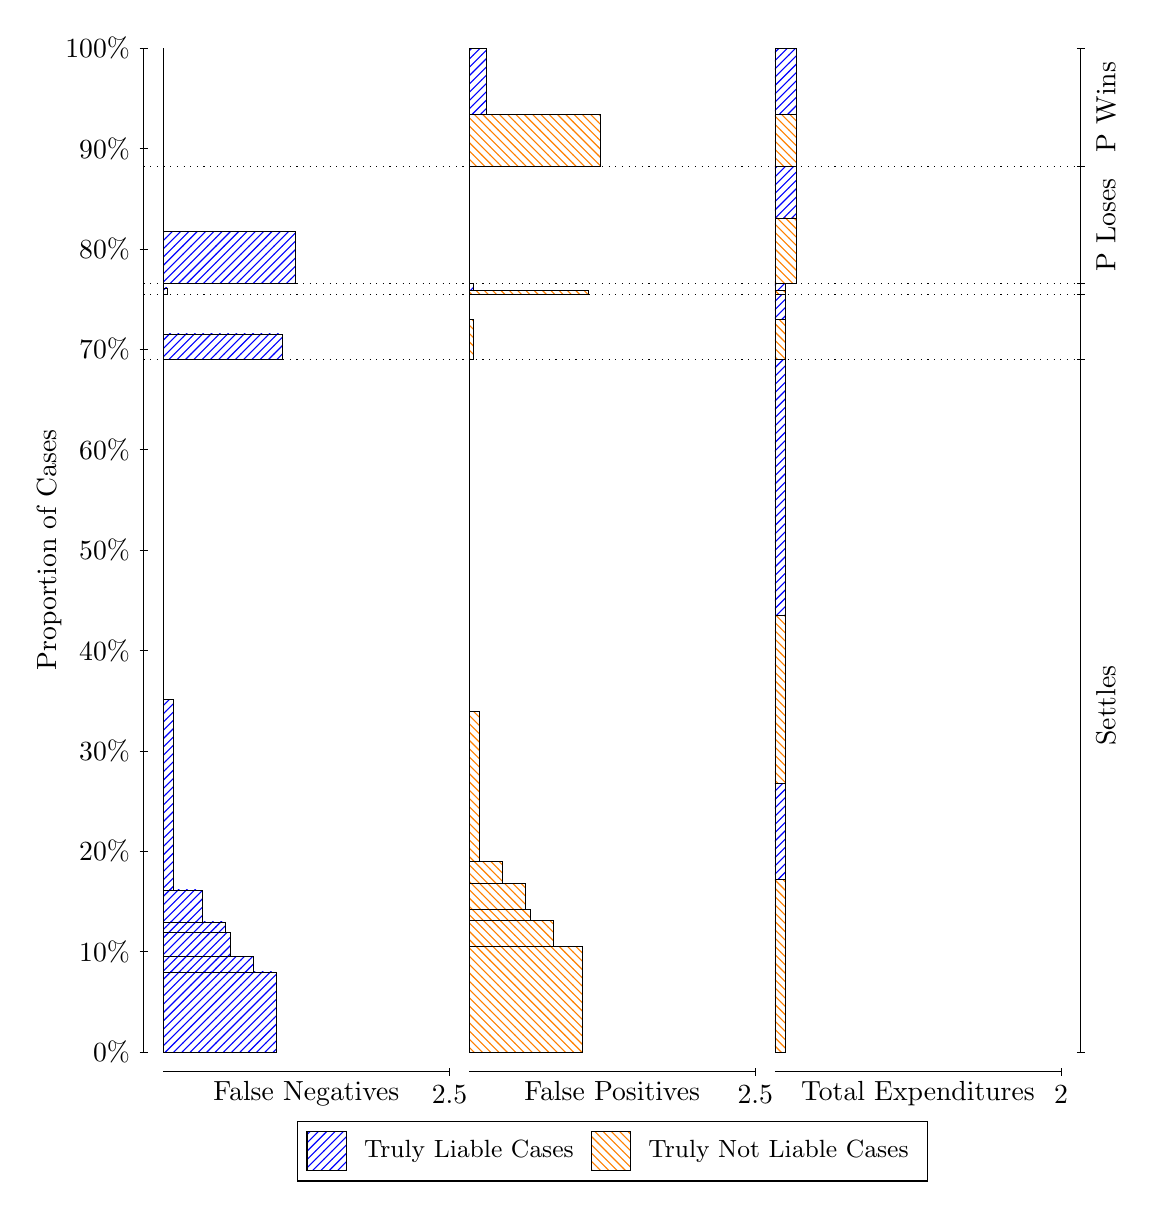
\begin{tikzpicture}
\draw[black, very thin] (1.5,1.75) -- (1.5,14.5);
\node[rotate=90, text=black, anchor=center] at (0.3, 8.125) {Proportion of Cases};
\draw[black, very thin] (1.45,1.75) -- (1.55,1.75);
\node[text=black, anchor=east] at (1.45, 1.75) {0\%};
\draw[black, very thin] (1.45,3.025) -- (1.55,3.025);
\node[text=black, anchor=east] at (1.45, 3.025) {10\%};
\draw[black, very thin] (1.45,4.3) -- (1.55,4.3);
\node[text=black, anchor=east] at (1.45, 4.3) {20\%};
\draw[black, very thin] (1.45,5.575) -- (1.55,5.575);
\node[text=black, anchor=east] at (1.45, 5.575) {30\%};
\draw[black, very thin] (1.45,6.85) -- (1.55,6.85);
\node[text=black, anchor=east] at (1.45, 6.85) {40\%};
\draw[black, very thin] (1.45,8.125) -- (1.55,8.125);
\node[text=black, anchor=east] at (1.45, 8.125) {50\%};
\draw[black, very thin] (1.45,9.4) -- (1.55,9.4);
\node[text=black, anchor=east] at (1.45, 9.4) {60\%};
\draw[black, very thin] (1.45,10.675) -- (1.55,10.675);
\node[text=black, anchor=east] at (1.45, 10.675) {70\%};
\draw[black, very thin] (1.45,11.95) -- (1.55,11.95);
\node[text=black, anchor=east] at (1.45, 11.95) {80\%};
\draw[black, very thin] (1.45,13.225) -- (1.55,13.225);
\node[text=black, anchor=east] at (1.45, 13.225) {90\%};
\draw[black, very thin] (1.45,14.5) -- (1.55,14.5);
\node[text=black, anchor=east] at (1.45, 14.5) {100\%};

\draw[black, very thin] (13.4,1.75) -- (13.4,14.5);
\draw[black, very thin] (13.35,1.75) -- (13.45,1.75);
\node[anchor=west] at (13.35, 1.75) {};
\draw[black, very thin] (13.35,10.55) -- (13.45,10.55);
\node[anchor=west] at (13.35, 10.55) {};
\draw[black, very thin] (13.35,11.368) -- (13.45,11.368);
\node[anchor=west] at (13.35, 11.368) {};
\draw[black, very thin] (13.35,11.511) -- (13.45,11.511);
\node[anchor=west] at (13.35, 11.511) {};
\draw[black, very thin] (13.35,13.001) -- (13.45,13.001);
\node[anchor=west] at (13.35, 13.001) {};
\draw[black, very thin] (13.35,14.5) -- (13.45,14.5);
\node[anchor=west] at (13.35, 14.5) {};

\draw[black, very thin, pattern color=blue, pattern=north east lines] (1.75,1.75) rectangle (3.1852,2.7659);
\draw[black, very thin, pattern color=blue, pattern=north east lines] (1.75,2.7659) rectangle (2.8945,2.9672);
\draw[black, very thin, pattern color=blue, pattern=north east lines] (1.75,2.9672) rectangle (2.6038,3.2727);
\draw[black, very thin, pattern color=blue, pattern=north east lines] (1.75,3.2727) rectangle (2.5312,3.4024);
\draw[black, very thin, pattern color=blue, pattern=north east lines] (1.75,3.4024) rectangle (2.2405,3.809);
\draw[black, very thin, pattern color=blue, pattern=north east lines] (1.75,3.809) rectangle (1.8772,6.223);
\draw[black, very thin, pattern color=orange, pattern=north west lines] (1.75,6.223) rectangle (1.75,10.55);
\draw[black, very thin, pattern color=blue, pattern=north east lines] (1.75,10.55) rectangle (3.2578,10.869);
\draw[black, very thin, pattern color=orange, pattern=north west lines] (1.75,10.869) rectangle (1.75,11.368);
\draw[black, very thin, pattern color=blue, pattern=north east lines] (1.75,11.368) rectangle (1.8045,11.455);
\draw[black, very thin, pattern color=orange, pattern=north west lines] (1.75,11.455) rectangle (1.75,11.511);
\draw[black, very thin, pattern color=blue, pattern=north east lines] (1.75,11.511) rectangle (3.4213,12.169);
\draw[black, very thin, pattern color=orange, pattern=north west lines] (1.75,12.169) rectangle (1.75,13.001);
\draw[black, very thin, pattern color=orange, pattern=north west lines] (1.75,13.001) rectangle (1.75,13.662);
\draw[black, very thin, pattern color=blue, pattern=north east lines] (1.75,13.662) rectangle (1.75,14.5);
\draw[black, very thin, pattern color=orange, pattern=north west lines] (5.6333,1.75) rectangle (7.0685,3.095);
\draw[black, very thin, pattern color=orange, pattern=north west lines] (5.6333,3.095) rectangle (6.7052,3.4212);
\draw[black, very thin, pattern color=orange, pattern=north west lines] (5.6333,3.4212) rectangle (6.4145,3.5615);
\draw[black, very thin, pattern color=orange, pattern=north west lines] (5.6333,3.5615) rectangle (6.3418,3.8864);
\draw[black, very thin, pattern color=orange, pattern=north west lines] (5.6333,3.8864) rectangle (6.0512,4.1697);
\draw[black, very thin, pattern color=orange, pattern=north west lines] (5.6333,4.1697) rectangle (5.7605,6.077);
\draw[black, very thin, pattern color=blue, pattern=north east lines] (5.6333,6.077) rectangle (5.6333,10.55);
\draw[black, very thin, pattern color=orange, pattern=north west lines] (5.6333,10.55) rectangle (5.6878,11.049);
\draw[black, very thin, pattern color=blue, pattern=north east lines] (5.6333,11.049) rectangle (5.6333,11.368);
\draw[black, very thin, pattern color=orange, pattern=north west lines] (5.6333,11.368) rectangle (7.1412,11.424);
\draw[black, very thin, pattern color=blue, pattern=north east lines] (5.6333,11.424) rectangle (5.6878,11.511);
\draw[black, very thin, pattern color=orange, pattern=north west lines] (5.6333,11.511) rectangle (5.6333,12.343);
\draw[black, very thin, pattern color=blue, pattern=north east lines] (5.6333,12.343) rectangle (5.6333,13.001);
\draw[black, very thin, pattern color=orange, pattern=north west lines] (5.6333,13.001) rectangle (7.3047,13.662);
\draw[black, very thin, pattern color=blue, pattern=north east lines] (5.6333,13.662) rectangle (5.8513,14.5);
\draw[black, very thin, pattern color=orange, pattern=north west lines] (9.5167,1.75) rectangle (9.6529,3.9405);
\draw[black, very thin, pattern color=blue, pattern=north east lines] (9.5167,3.9405) rectangle (9.6529,5.1577);
\draw[black, very thin, pattern color=orange, pattern=north west lines] (9.5167,5.1577) rectangle (9.6529,7.2942);
\draw[black, very thin, pattern color=blue, pattern=north east lines] (9.5167,7.2942) rectangle (9.6529,10.55);
\draw[black, very thin, pattern color=orange, pattern=north west lines] (9.5167,10.55) rectangle (9.6529,11.049);
\draw[black, very thin, pattern color=blue, pattern=north east lines] (9.5167,11.049) rectangle (9.6529,11.368);
\draw[black, very thin, pattern color=orange, pattern=north west lines] (9.5167,11.368) rectangle (9.6529,11.424);
\draw[black, very thin, pattern color=blue, pattern=north east lines] (9.5167,11.424) rectangle (9.6529,11.511);
\draw[black, very thin, pattern color=orange, pattern=north west lines] (9.5167,11.511) rectangle (9.7892,12.343);
\draw[black, very thin, pattern color=blue, pattern=north east lines] (9.5167,12.343) rectangle (9.7892,13.001);
\draw[black, very thin, pattern color=orange, pattern=north west lines] (9.5167,13.001) rectangle (9.7892,13.662);
\draw[black, very thin, pattern color=blue, pattern=north east lines] (9.5167,13.662) rectangle (9.7892,14.5);
\draw[black, dotted] (1.5,10.55) -- (13.4,10.55);
\draw[black, dotted] (1.5,11.368) -- (13.4,11.368);
\draw[black, dotted] (1.5,11.511) -- (13.4,11.511);
\draw[black, dotted] (1.5,13.001) -- (13.4,13.001);
\draw[black, very thin] (1.75,1.5) -- (5.3833,1.5);
\node[text=black, anchor=north] at (3.5667, 1.5) {False Negatives};
\draw[black, very thin] (5.3833,1.45) -- (5.3833,1.55);
\node[text=black, anchor=north] at (5.3833, 1.45) {2.5};

\draw[black, very thin] (5.6333,1.5) -- (9.2667,1.5);
\node[text=black, anchor=north] at (7.45, 1.5) {False Positives};
\draw[black, very thin] (9.2667,1.45) -- (9.2667,1.55);
\node[text=black, anchor=north] at (9.2667, 1.45) {2.5};

\draw[black, very thin] (9.5167,1.5) -- (13.15,1.5);
\node[text=black, anchor=north] at (11.333, 1.5) {Total Expenditures};
\draw[black, very thin] (13.15,1.45) -- (13.15,1.55);
\node[text=black, anchor=north] at (13.15, 1.45) {2};

\node[text=black, centered, rotate=90] at (13.72, 6.15) {Settles};


\node[text=black, centered, rotate=90] at (13.72, 12.256) {P Loses};
\node[text=black, centered, rotate=90] at (13.72, 13.75) {P Wins};

\draw (7.449999999999999,1.5) node[draw=none] (baseCoordinate) {};
\begin{scope}[align=center]
        \matrix[scale=0.5, draw=black, below=0.5cm of baseCoordinate, nodes={draw}, column sep=0.1cm]{
            \node[rectangle, draw, minimum width=0.5cm, minimum height=0.5cm, pattern color=blue, pattern=north east lines] {}; &
            \node[draw=none, font=\small, text=black] (B) {Truly Liable Cases}; &
            \node[rectangle, draw, minimum width=0.5cm, minimum height=0.5cm, pattern color=orange, pattern=north west lines] {}; &
            \node[draw=none, font=\small, text=black] (B) {Truly Not Liable Cases}; \\
            };
\end{scope}

\end{tikzpicture}
\end{document}